%%! program = pdflatex
%
%\documentclass[12pt,a4paper]{article} 
%\usepackage{arc-dp}
%\usepackage{amsfonts}
%\usepackage{amsmath}
%\usepackage{graphicx}
%\usepackage{times}
%\usepackage{setspace}
%\usepackage{fancyhdr}
%\usepackage{color}
%\usepackage[normalem]{ulem}
%\usepackage{subfig}
%\usepackage{float}
%\usepackage{caption}
%\usepackage{array}
%\usepackage{pgfgantt}
%\usepackage{url}
%\usepackage{enumitem}
%\usepackage{subfig}
%\usepackage{pgfgantt}
%\usepackage{wrapfig}
%\usepackage{enumitem}
%
%\usepackage{booktabs} % for spacing tables
%\usepackage{tabularx} % auto table sizing
%\usepackage{multirow} % table multirow
%\usepackage{soul}
%
%%\usepackage{epsf}
%%\usepackage{fancyheadings}
%%\usepackage{subfigure}
%%\usepackage{pst-gantt}
%%\usepackage{tweaklist}
%
%\newcolumntype{L}[1]{>{\raggedright\let\newline\\\arraybackslash\hspace{0pt}}m{#1}}
%\newcolumntype{C}[1]{>{\centering\let\newline\\\arraybackslash\hspace{0pt}}m{#1}}
%\newcolumntype{R}[1]{>{\raggedleft\let\newline\\\arraybackslash\hspace{0pt}}m{#1}}
%
%\let\OLDthebibliography\thebibliography
%\renewcommand\thebibliography[1]{
%  \OLDthebibliography{#1}
%  \setlength{\parskip}{1pt}
%  \setlength{\itemsep}{1pt plus 0.3ex}
%}
%
%
%%\renewcommand{\enumhook}{\setlength{\topsep}{0pt}%
% % \setlength{\itemsep}{-2mm}}
%%\renewcommand{\itemhook}{\setlength{\topsep}{0pt}%
%%  \setlength{\itemsep}{-2mm}}
%  %%%%%UNCOMMENT THE NEXT COMMAND IF NEEDED
%%\renewcommand{\descripthook}{\setlength{\topsep}{0pt}%
%%  \setlength{\itemsep}{-2mm}}
%
%%\pagestyle{fancy}
%
%%\input{psfig.sty}
%\newcommand{\todo}[1]{\textcolor{red}{#1}}
%\newcommand{\rules}[1]{\textcolor{blue}{#1}}
%\newcommand{\pset}{ {\rm P} \! \! \! {\rm P} }
%\date{}
%%\include{psfig}
%\remove{
%\topmargin -15mm
%\headheight 0pt
%\headsep 0pt
%\textheight 285mm
%\oddsidemargin -15mm
%\evensidemargin -15mm
%\textwidth 190mm
%\columnsep 10mm
%\marginparwidth 0pt
%\marginparsep 0pt
%}
%
%\usepackage[top=0.5cm, bottom=0.5cm, left=0.5cm, right=0.5cm]{geometry}
%\parindent=4mm
%\parskip=0.2mm
%
%%\usepackage{geometry} % see geometry.pdf on how to lay out the page. There's lots.
%%\geometry{a4paper} % or letter or a5paper or ... etc
%% \geometry{landscape} % rotated page geometry
%
%
%%\linespread{1.5}
%
%\newcommand*{\TitleFont}{%
%      \usefont{\encodingdefault}{\rmdefault}{b}{n}%
%      \fontsize{12}{12}%
%      \selectfont}
%
%\title{A unified accessible platform for integration of urban analytics and human thermal comfort modelling}
%%\author{}
%\date{} % delete this line to display the current date
%
%%%% BEGIN DOCUMENT
%\begin{document}
%\rmfamily
%\date{}


\noindent \textbf{F18-ROPE-Details of the participant's academic career and opportunities for research, evidence of research impact and contributions to the field, including those most relevant to this application }\\ \noindent 





\subsection*{\TitleFont Amount of Time as an Active Researcher}

~~~~I was awarded my PhD on urban micro-climate modelling from the School of Earth, Atmosphere and Environment at Monash University in March 2017. I have been an active researcher (at 1.0 FTE) for 4 years and 10 months post-PhD without interruption.

\subsection*{\TitleFont Research Opportunities}

\subsubsection*{\textbf{Academic career}}



~~~~Following a 13 year industry career as a senior and consulting level software engineer (most significantly 8 years at LexisNexis/Reed Elsevier), I returned to university. This previous career has proven highly transferable to my academic research career. It gave me a high level of expertise in software development and design and proficiency in many computer languages (including C++, Python, FORTRAN, and especially Java). I also gained years of experience in project development and management, guiding multi-year projects, developed by globally distributed teams, and delivered to multiple business units around the global. This experience has been directly transferable to managing large research programs, working with remote collaborators, and supervising students.

My post graduate academic career started at the School of Earth, Atmosphere \& Environment  at Monash University. My Master's final semester research project was an observational and modelling study examining the micro-climate of mixed urban and parkland environments which led to engagement by the CRC for Water Sensitive Cities to write a report recommending (but not finding an existing) micro-climate model suitable for thermal comfort impact assessments of water sensitive urban design (especially urban vegetation and water features). My PhD at Monash University followed from this, designing and building this (missing) model. The models VTUF-3D and TARGET resulted from this PhD research and subsequent collaborations with other researchers at Monash. I also designed and built the user interface for the Monash University Simple Climate Model (MSCM) with A/Prof. Dietmar Dommenget (F20, referred articles \#7). This web-based interface (F20, additional research outputs \#17) is a teaching tool that allows students to interactively study the interactions of physical processes in the global climate system through the results of more than a 1000 different model experiments of the Globally Resolved Energy Balance (GREB) model.

My post-doctoral career, at times, has been split (50/50) between two research fellow positions (funded separately) but that encompass research areas that use modelling and computational techniques to examine urban areas for health impacts. One of these position was a 2 year 0.5 FTE research contract (subcontracted through the University of Melbourne) as a Research Fellow and urban climate modelling scientist with Monash University and the CRC for Water Sensitive Cities. My achievements in urban climate model development, even at an early research career stage, have led to recognition as an expert in vegetation and human thermal comfort modelling, leading to this external funding from the CRC for Water Sensitive Cities to further develop this work and consult with local and state government. This role was split between 40\% research, 40\% tool development, and 20\% consulting. 

The research portion was largely devoted to assessments of urban heat outcomes for different urban infill development scenarios. I designed and performed an urban heat analysis of a number of different green field development scenarios in Sunbury for the CRC, especially considering water sensitive (and climate sensitive) urban design. This resulted in a report for the CRC, "Estimating the economic benefits of Urban Heat Island mitigation – Biophysical Aspects" (F20, additional research outputs \#9). Additional modelling analysis of infill development typologies in a number of Australian cities resulted in three additional reports, the `Infill Performance Evaluation Framework', the `Knutsford Urban Heat Modelling Report', and the `Salisbury case study final report: water sensitive outcomes for infill development'. Finally, I wrote the report `Managing urban heat in water sensitive cities: research and policy responses' to summarise the heat mitigation research of the CRC over its eight year program. These reports are additional research outputs \#1-5.

The tool development was devoted to continued development of my urban climate models VTUF-3D and TARGET and their integration with the CRC's scenario planning support tool. I also used this opportunity to improve the performance and usability of my climate models. This is important as very few models can quantify the human thermal benefits of urban green and blue space, especially accounting for cooling effects of vegetation and water evaporation, but often the complexity of configuring, running, and interpreting modelling means this knowledge is out of reach for most potential users.



The consulting included urban heat modelling for state and local government, often joint projects with consulting companies such as GHD. For example, projects resulted in contributions of urban heat assessments to the Urban Ecology Strategy for Fishermans Bend for the Victoria Department of Environment, Land, Water \& Planning (DELWP) and serving on the science panel for the development of the Cool Suburbs Tool for the Western Sydney Regional Organisation of Councils (WSROC). Additional projects include a microclimate assessment for the ACT government and assessments of future heat vulnerability for the Queensland DES/QFES.


\subsubsection*{\textbf{Current roles}}


~~~~My current position is as a Research Fellow (research only)  with the Transport, Heath, and Urban Design (THUD) Research Lab in the Faculty of Architecture, Building, and Planning at the University of Melbourne. This involves research using innovative technologies (artificial intelligence, big data analysis, agent-based modelling, computer vision techniques as well as more traditional statistical methods) to examine multiple aspects of urban areas such as transport networks, urban features, and urban heat and impacts on public health. Building on my PhD research and the position with the CRC, this position incorporates a wide range of disciplines and applies the development and application of modelling to public heath problems. For example, this modelling was applied to a wide range of applications, including modelling of the COVID-19 roadmap for Victoria, creating inventories of cycling infrastructure from remote sensing images, and assessing the impacts of global cities typologies on road injuries. In addition, my software development skills and computer vision technical knowledge has proven highly beneficial to undertaking research across multiple disciplines, leading to new innovations in quantifying health impacts of urban design and transportation infrastructure. This has led to my role as a key contributor to the research lab.

My initial task in THUD was to organise and write an ARC Linkage application, 'A Multi-criteria Design Platform to Facilitate Active School Journeys', quantifying topography, street network connectivity, traffic risk, pollution levels, and thermal comfort. I was not a named participant but the application was submitted in December 2017 (and resubmitted and funded in 2020). I co-developed the neural network clustering and analysis technique used in the lab's recent Lancet Planetary Health publication. This allowed the identification of city types from map segments from the 1700 largest global cities at higher risk of road trauma. This method was expanded in a more recent publication (with myself as first author) in Urban Science to also include street view imagery and satellite imagery to derive urban typologies. Also, in conjunction with other lab collaborators, I developed a method to identify neighbourhood typologies (`block typologies') using self organising maps to cluster metrics extracted from map segments. All three of these projects were used as the base methodology for our lab's current \$1.3 million NHMRC/UKRI research project. My contribution to the lab is also represented in many of the 10 journal publications I co-authored with the lab in the last 4 years.

My expertise in urban heat modelling and computer vision techniques have led to me being sought out to participate as a co-investigator a \$422,000 ARC Discovery (fully detailed below) to create cycling risk exposure models from satellite and street view imagery and from Strava data and traffic cameras. I am also a co-investigator on an awarded 453,764 CHF Swiss National Science Foundation grant `Heat-Down: Integrated modelling of stormwater and urban heat for cooling cities' headed by Dr. Jo\~{a}o P. Leit\~{a}o (Eawag) and Dr. Peter M. Bach (ETH Zurich) based on my TARGET model. I have also built on an ongoing collaboration with the UNSW City Futures Research Centre with a recently submitted application for the AURIN High Impact Projects 2021, `Climate Resilient and Just Cities: Data for Research and Practice' led by Dr. Negin Nazarian.

At the University of Melbourne, Prof. Mark Stevenson (professor of Urban Transport and Public Health and NHMRC Research Fellow) supervises my other position and along with other members of the lab (especially Dr. Jason Thompson, the senior research fellow in the lab) provides valuable mentoring. Through my academic career, I have been fortunate to receive excellent mentoring and career guidance. My PhD was supervised by Prof. Nigel Tapper (Monash University; current president of The International Association for Urban Climate) and Dr. Andrew Coutts (Monash University; a leading urban climate researcher). Prof. Tapper remains a frequent collaborator and co-supervisor of honours and PhD students. 




\subsection*{\TitleFont Research Achievements and Contributions}

\textbf{How my research has led to advances in knowledge in the field. How will my achievements contribute to the application:}


As an early-career researcher, I have quickly built a large body of work. These research achievements include a number of urban climate models able to examine urban heat mitigation strategies at local and micro-scales and make predictions of human thermal stress. These models have been adopted by other researchers and consultants. My knowledge about modelling and model development has led to being included in research projects and grant applications to further develop these models and contribute to the development of other models. In addition, methods that I have developed using computer vision techniques to cluster similar types of urban areas and examine the links of the design to public health outcomes and have formed the basis of successful grant applications and research papers. These techniques and the results from them (especially those around urban heat) are currently being utilised by state and local governments to formulate appropriate public health measures.

After my industry career and PhD candidacy, I have focused on building and improving my track record as a researcher. Despite having completed my PhD by thesis and as a result my research has only started to be published in 2018, when comparing with other researchers in urban climate modelling and model development at similar stages of their careers, my publication output compares favourably (Figure \ref{fig:benchmark}). When comparing citation counts, my record shows a rapidly rising trajectory in the last four years (in Google Scholar, 13 in 2019, 60 in 2020, and 90 in 2021), but it should also be considered that citations take a number of years to accumulate.



\begin{wrapfigure}{r}{0.65\textwidth}
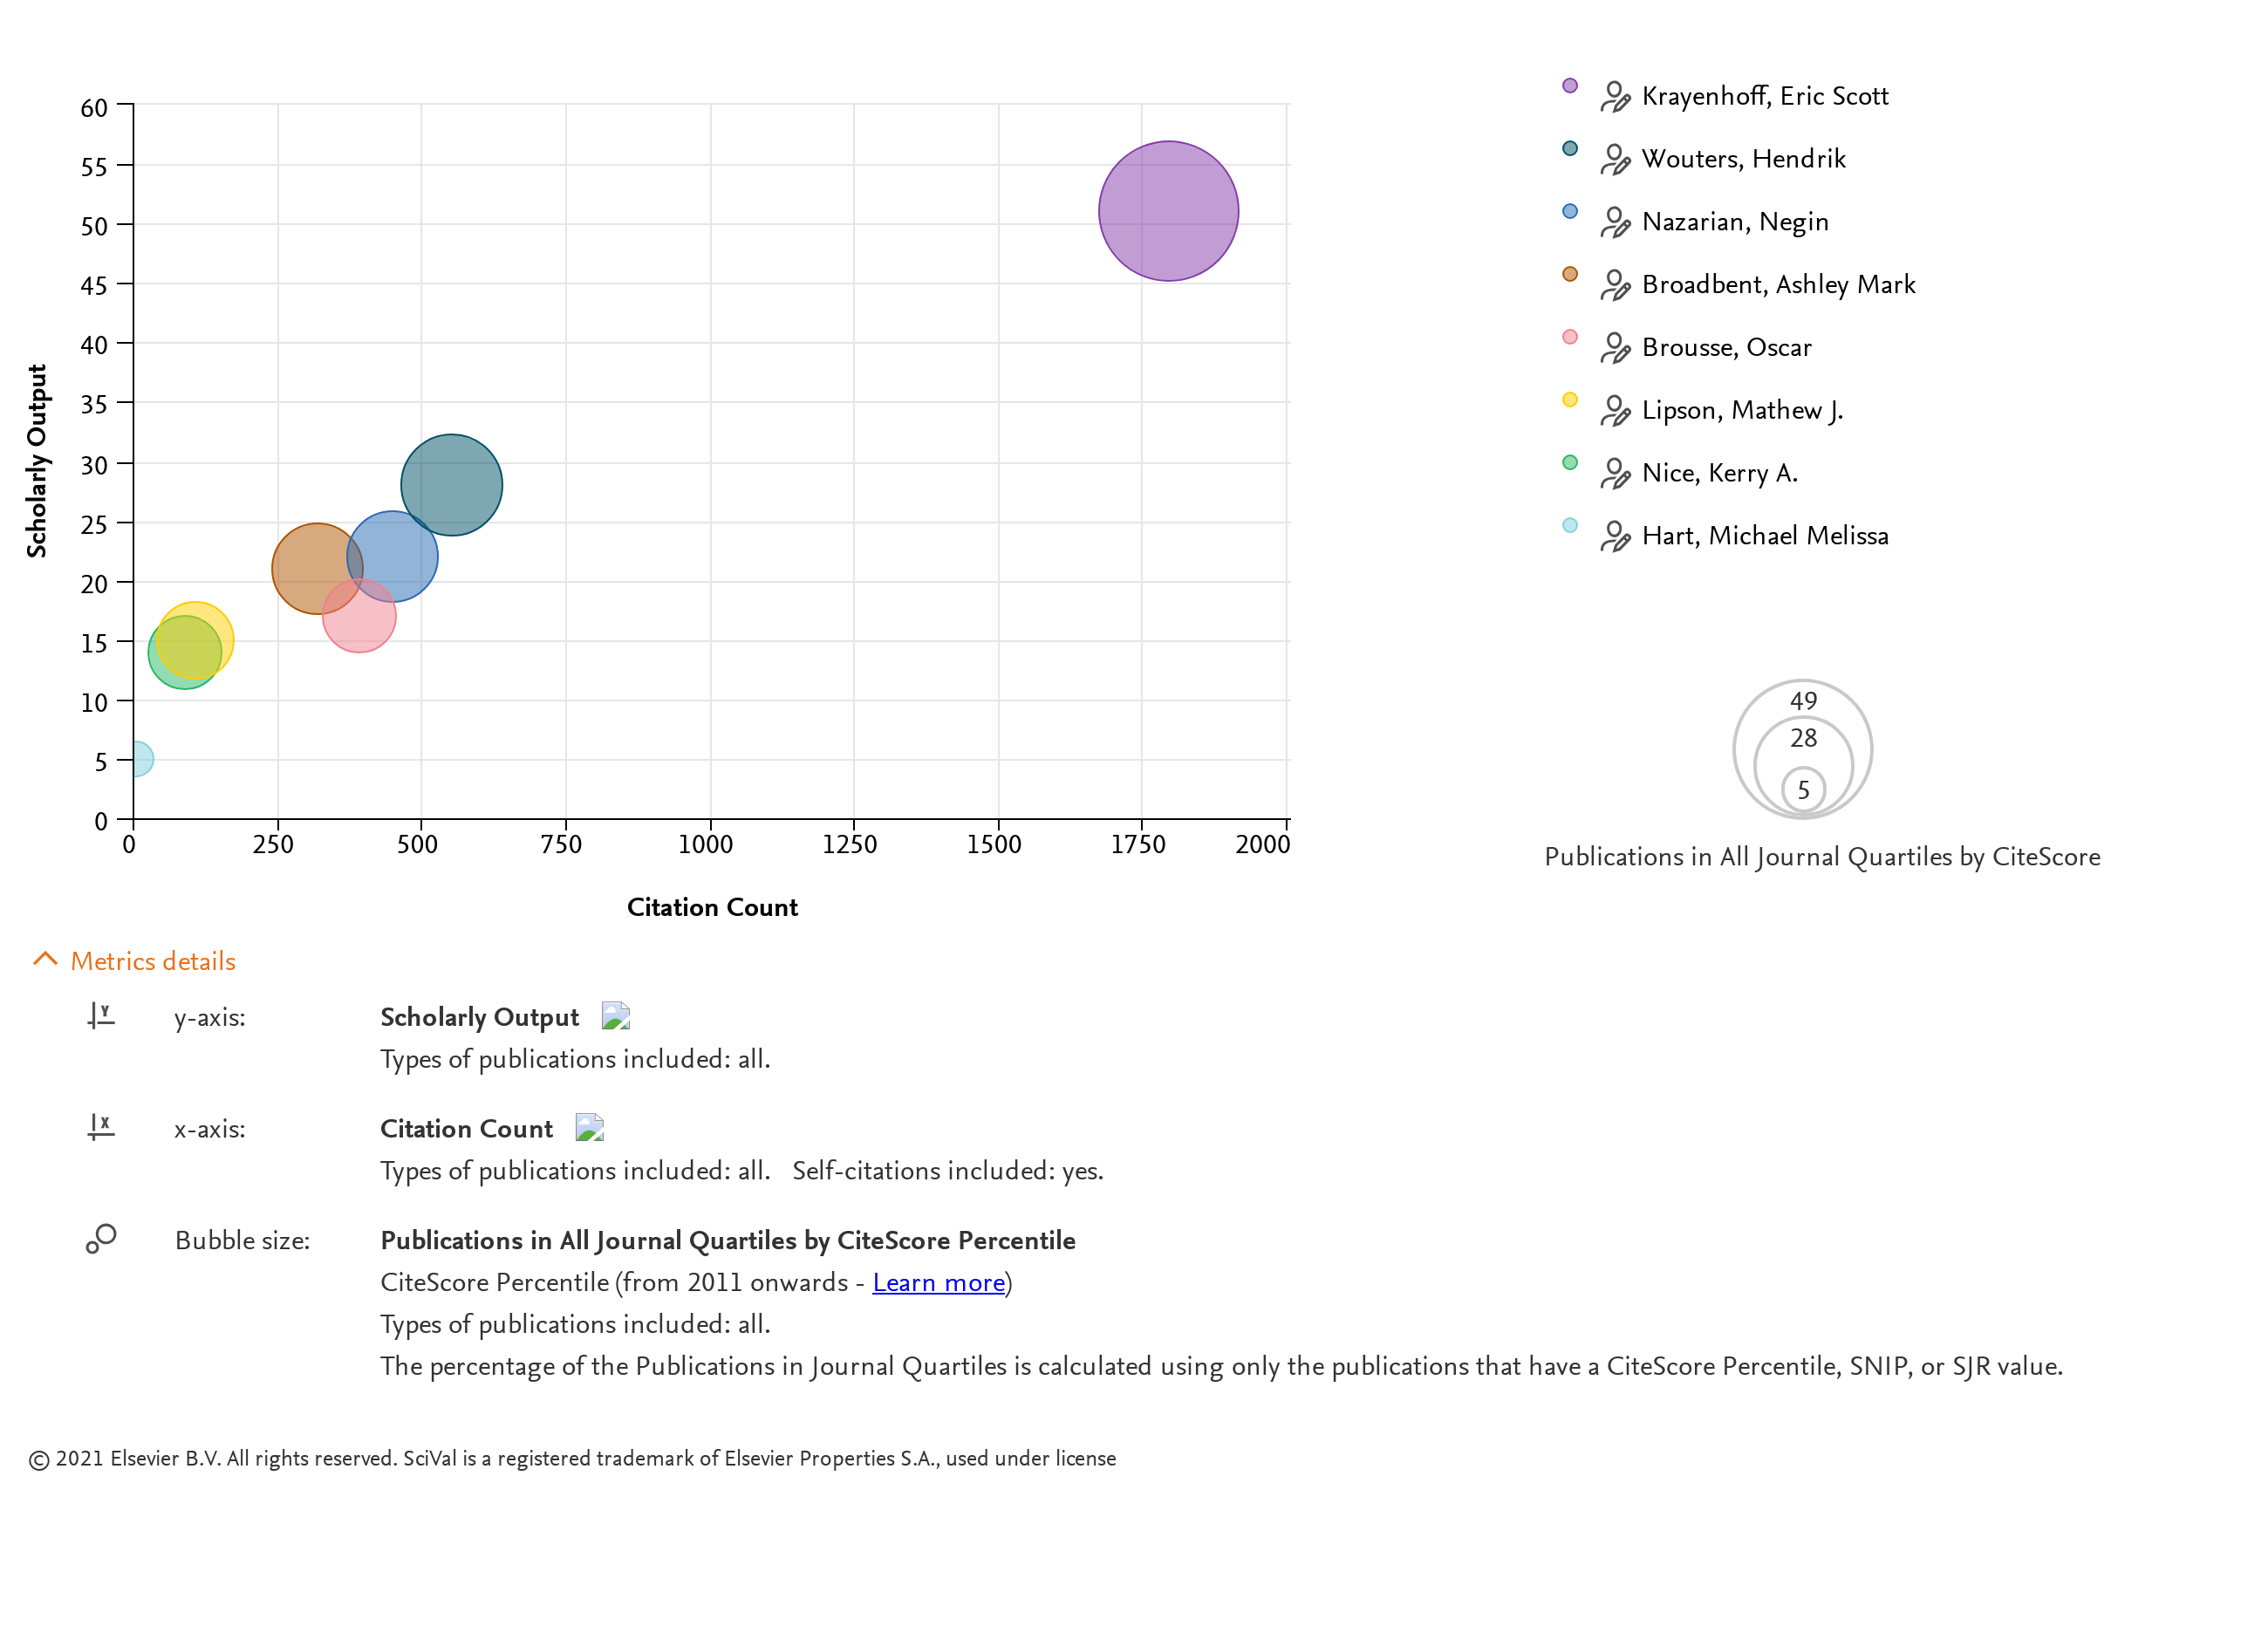
\includegraphics[trim={20 800 150 20},clip,scale=0.12]{metrics/K-Nice-2-2021.png}
\caption{Benchmarking of my publication output in top 10\% journals (by CiteScore percentile) compared to well-regarded researchers in urban climate modelling and model development at similar stages of their careers. Y-axis: All types of publications included. Bubble size: CiteScore percentile (from 2011 onward) (Source: Elsevier SciVal).}
\label{fig:benchmark}
\end{wrapfigure}


The first stage of my academic career has been in urban climate modelling, the topic of my PhD. The model I developed in my PhD, VTUF-3D remains one of the few models able to assess the cooling impacts of urban vegetation at a micro-scale, and has led to further collaborations and model development as well as a large engagement. My PhD thesis, from which the journal article was developed, has had over 2,000 reads. Three additional climate models, TARGET, UT\&C, and MSCM-DB, have been co-developed through collaborations. In a collaboration (F20, top 10 \#8), have explored the state of the art in modelling (including my VTUF-3D model) outdoor mean radiant temperatures, a key parameter for predicting heat stress, and found circumstances where VTUF-3D and ENVI-met successfully model this parameter and where they encounter challenges. 

My recent paper in Sustainable Cities and Society, `Estimating the cooling potential of irrigating green spaces' is directly related to this DECRA application. In addition, my research in urban heat has also included wider multidisciplinary applications of (and a framework around) water usage and urban design on both urban heat and other issues of urban liveability that were presented at the State of Australian Cities conference (\#2 below). I have utilised computer vision techniques in support of urban climate modelling. This led to a method to more accurately detect sky pixels (a preliminary step in calculating sky view factors) using a range of urban imagery types (F20, top 10 \#4). I presented methods to utilise urban morphology databases (such as WUDAPT) in conjunction with micro-climate modelling to target heat mitigation strategies and the beginning steps to discover and define micro-climate zones at the European Geosciences Union conference EGU2020 (\#3 below). This has been expanded to an (in-progress) collaboration with researchers at UNSW to isolate the impacts of urban form and fabric from geography on heat mitigation strategies.

While my expertise in urban climate and urban climate modelling have the most direct link to the successful delivery of this project, much of my recent research has involved the use of artificial intelligence and machine learning. These techniques can be applied to urban climate questions as well. The \$30,000 2020 Melbourne Energy Institute grant resulted in a study (currently in review with Atmospheric Pollution Research) using XGBoost to quantify the effects of human activity (reduced during COVID-19) on key pollutants (NO$_{2}$, PM$_{2.5}$, PM$_{10}$, and O$_{3}$) across 700 global cities. Other research has included using neural networks to cluster the largest 1700 global cities using millions of maps and examine the impact of urban design types on road trauma, as well as adding additional imagery types (satellite and street view) to the maps to construct urban typologies based on features discovered in the imagery. I've used other types of artificial intelligence, generative adversarial networks, to transform street level and satellite imagery from areas with poor health outcomes into new imagery, providing insights into the urban factors leading to these poor outcomes. Finally, I have used deep autoencoder extracted features from satellite imagery of all the intersections in Australia to identify safe intersection design. 

In addition, my record of publication in high impact journals have also given me an understanding of complex review processes and required engagement in international-level debates. The Computer-Aided Civil and Infrastructure Engineering publication required satisfying 10 reviewers. The Lancet Planetary Health publication, with a multi-year review process and an excess of 10 reviewers, proved even more challenging. Numerous editorials are published in public health about the need to develop and utilise new techniques and multi-disciplinary approaches, but actually submitting this work requires overcoming large amounts of resistance to moving beyond what has always been done.

I have presented my research at 8 international conferences and 7 national conferences with 3 of those as invited talks. My research has also been featured in 5 collaborative presentations at 5 international conferences (1 as an invited talk). 

The following conference presentations and conference papers are most strongly related to this DECRA application (i.e. climate model development, human thermal comfort modelling, and the collection of urban morphology information through databases and extraction from urban imagery).

\begin{list}{}{}
\itemsep-0.5em

\item [1.] G\'{a}l, C. V and \textbf{Nice, K. A.} ‘Mean radiant temperature modeling outdoors: A comparison of three approaches’, in \textit{100th Annual Meeting of the American Meteorological Society (AMS) jointly with the 15th Symposium on the Urban Environment}, 2020. 
\item [2.] Todorovic, Tatjana, London, Geoffrey, Bertram, Nigel, Sainsbury, Oscar, Renouf, Marguerite A, \textbf{Nice, Kerry A} and Kenway, Steven J. 2019. ‘Models for water sensitive middle suburban infill development’, in\textit{ 9th State of Australian Cities National Conference, 30 November - 5 December 2019, Perth, Western Australia}. doi: 10.25916/5efa774bda643. 
\item [3.] \textbf{Nice, K. A.}, Targeted urban heat mitigation strategies using urban morphology databases and micro-climate modelling to examine the urban heat profile. \textit{EGU General Assembly 2020}.

\end{list}

Further other research outputs support my expertise in urban climates, urban typology clustering and urban analytics.
\begin{list}{}{}
\itemsep-0.5em
\item [4.] \textbf{Nice, K. A.}, Climate science context around urban cooling. In: \textit{4th Water Sensitive Cities Conference 2019, Brisbane}. \textbf{Invited talk.}
\item [5.] \textbf{Nice, K. A.}, Urban Greening for improved human thermal comfort. In: \textit{202020 Vision, The Green Light Tour, 2018, Adelaide}. \textbf{Invited talk.}
\item [6.] \textbf{Nice, K. A.}, Designing liveable cities through heat mitigation: tools to translate knowledge into design. In: \textit{3rd Water Sensitive Cities Conference, 2017, Perth.} \textbf{Invited talk.}
\item [7.] \textbf{Nice, K.A.}, The Nature of Human Settlement: Building an understanding of high performance city design. In: \textit{UrbanSys2019/2019 Conference on Complex Systems, Singapore.}
\end{list}

I have developed a strong collaborative network (within my universities, Australia, and internationally), and developed a strong research direction based on modelling and quantifying urban systems. This rapid upward trajectory has been strongly enabled by a previous long career in industry and software engineering that required the ability to develop and organise large projects, solve problems, and build the tools necessary to deliver results. This combination of extensive experience in computing techniques with deep urban climate and urban climate modelling development knowledge demonstrate that I am the ideal researcher to undertake and deliver this project.


\textbf{Invited keynote and speaker addresses:}

I have presented my research at 8 international and 7 (3 invited, \#4, \#5, and \#6 above) national conferences since 2012. Three of these have been at the International Conference on Urban Climate (ICUC), the leading conference for urban climate. Two of these ICUC talks were about my VTUF-3D model and one was about using computer vision techniques and Google Street View to discover urban morphology parameters (namely sky view factors). Two recent international conference presentations have been on the topic of deriving urban typologies through big data urban imagery datasets and machine learning and computer vision. I have given three invited presentations on the topics of urban heat and designing heat mitigation strategies at the 3rd and 4th Water Sensitive Cities Conferences in Perth and Brisbane and in the 202020 Vision Green Light Tour in Adelaide (202020 Vision is now Greener Spaces Better Places). I have also been invited to present five guest lectures at Monash University and the University of Melbourne on the topic of urban climate modelling and the urban heat benefits of water sensitive urban design. 

\textbf{Research income:}

I have secured AUD \$1,207,910, GBP \textsterling479,387, and 453,764 CHF in research income through competitive grants over the last five years. This demonstrates my capacity to secure funding across a wide range of research areas in collaboration with other Australian and international researchers and delivering publications and reports from these projects.

\begin{itemize}
\item In 2016 I was awarded the \$10,000 Graham Treloar Early Career Researcher Fellowship (The University of Melbourne Faculty of Architecture, Building and Planning) for the development of the project `Urban canyon mean radiant temperatures predictions through mining Google Street View imagery and neural network machine learning'. The outcome from this project was published in career-best publication \#4.

\item I am a Chief Investigator on the AUD \$608,910 (and GBP \textsterling479,387) 2020-2023 UKRI/NHMRC grant 1194959, `A Vision of Healthy Urban Design for NCD Prevention'. The methodology for this grant utilises neural networks and computer vision techniques to process large amounts of urban imagery to assess the impacts of urban design on non-communicable disease (NCD). This is a collaborative project between researchers at the University of Melbourne and Queen's University Belfast.

\item I secured a \$137,000 research contract with the CRC for Water Sensitive Cities as a specialist cohort in urban heat modelling. This contract was solicited by the CRC to provide urban heat expertise to the final two years of the CRC research program and provides two years of 0.5 FTE funding over 2019-2020. This funding has provided opportunities both to advance my model development work and work in collaboration with industry partners and local and state governments to develop urban heat mitigation strategies (as detailed in the benefits section below).

\item I am a Chief Investigator on a \$30,000 2020 Melbourne Energy Institute grant on `The effects of COVID-19 on reduced transport and emissions for global city typologies'. 

\item I am a Chief Investigator on the \$402,000 2021-2023 ARC Discovery DP210102089 `Sustainable mobility: city-wide exposure modelling to advance bicycling' grant headed by Dr Ben Beck (Monash University). This grant utilises my expertise in computer vision and machine learning to extract an inventory of cycling infrastructure from satellite and street view imagery. These inventories will be used to develop a platform for city-wide modelling of cycling exposure that can be applied globally.

\item I am a Partner Investigator on a 453,764 CHF 2021 Swiss National Science Foundation Project ID 200021\_201029, `Heat-Down: Integrated modelling of stormwater and urban heat for cooling cities'. My urban climate model, TARGET, will be upgraded and utilised to investigate heat mitigation strategies enabled by the use of stormwater.

\end{itemize}




\textbf{Research supervision, mentoring and advice:}


Student supervision of topics closely related to this project has provided experience in micro-climate observations of cooling through BGI features. I am currently co-supervising two PhD students in conjunction with Prof. Nigel Tapper (Monash) and A/Prof. Stephen Livesley (Melbourne). The student at Monash University/Southeast University is observing and modelling the cooling potential of irrigation of the runway buffer areas at Adelaide Airport. Another student at the University of Melbourne is looking at the cooling potential and energy balances of misting systems and irrigation of turf grass and trees. I am supervising one Honours student at Monash in conjunction with Prof. Nigel Tapper and Prof. Julie Arblaster, who will be modifying VTUF-3D to include the ability to model impervious surfaces watering based on an observation campaign.

I have also supervised the final capstone research projects for 11 Masters of IT (MIT) students at the University of Melbourne. Methods from 3 of these MIT projects were incorporated into the Urban Climate paper, listed above. In addition, methods from one other MIT project is currently being incorporated into a health/computer vision collaboration with researchers from Cambridge University. Finally, I have been invited to participate in 3 PhD review panels for the urban climate discipline.



\textbf{Benefits outside academia:}

My expertise in urban heat modelling has been utilised in a number of government consultations and planning reports in 2019-2021. I am currently consulting with the Department of Agriculture, Water and the Environment (DAWES) for the project 'Health cost impacts of urban heat amelioration through integrated water cycle management (IWCM) measures', a consortium through Marsden Jacob with a modelling team led by Prof. Nigel Tapper (Monash) with Dr. Andrew Coutts, and Dr. Matthias Demuzere (RUB) and a health team led by Prof. Peng Bi (University of Adelaide). Past projects include serving on the science advisory panel for Western Sydney Regional Organisation of Councils (WSROC) Cool Suburbs Rating and Accreditation tool, providing modelling and urban heat analysis for the Queensland Department of Environment and Science (DES), reports for urban heat impacts of infill development for South Australia (Salisbury, an Adelaide suburb) and Western Australia (the Perth suburb of Kutsford), urban heat assessments for the Fishermans Bend Urban Ecology Strategy for the Victorian government, and project work for the ACT government's micro-climate urban heat strategies.



\textbf{Other professional activities:}

I maintain memberships in the European Geosciences Union (EGU), The Australian Meteorological and Oceanographic Society (AMOS), The International Association for Urban Climate (ICUC), and the Complex Systems Society (CSS).

Article Referee Activities: In the past 5 years, I have performed 45 peer reviews for 17 leading climate and urban design journals, including Urban Climate, Theoretical and Applied Climatology, Sustainable Cities and Society, Environmental Science \& Technology, Environment and Planning B, Scientific Reports, Science of the Total Environment, Landscape and Urban Planning and am on the review board for Atmosphere.




%\end{document}
